\documentclass[11pt, oneside]{article}  
\usepackage{geometry}              
\usepackage{graphicx}			
\usepackage{amssymb}
\usepackage{mathtools}
\usepackage{enumerate}
\usepackage{comment}
\usepackage{amsmath, amssymb, amsthm, graphicx, hyperref}
\usepackage{enumitem}
\usepackage{fancyhdr}
\usepackage{multirow, multicol}
\usepackage{tikz}
\usepackage{relsize}
\usepackage{mathtools}
\usepackage{centernot}
\usepackage{cancel}
\usepackage{float}
\geometry{letterpaper}    

\title{Project Write Up\\
		\large Heart Attack Analysis\\
		\small Comparing Performances of Logistic Regression, SVM, and Neural Network Models to Predict Likelihood of Heart Attacks\\
		\large Spring 2021\\
		Prof. Sellie}
\author{JinWen Loh, Tom Liu}
\graphicspath{ {images/} }

\begin{document}
\maketitle
\section *{Overview}
The objective of this project is to analyze and compare the performances of three machine learning models to predict the likelihood that someone will get a heart attack. Said models are namely: Logistic Regression, SVMs, and Neural Networks. High (or good) performance is defined as having high accuracy when ran on the verification/test set.\\\\
Different variants of these models would also be tested to see if any differences could be observed from any changes. For example, we may perform different polynomial feature transformations for logistic regression, and note any differences in performance observed.\\\\
Apart from that, L2 regularization would also be applied to these variations in order to test if any improvements in performance could be observed.\\\\

\section*{Analyzing Data}
The following is the data we will be analyzing:
\begin{itemize}
    \item Age : Age of the patient

    \item Sex : Sex of the patient

    \item exang: exercise induced angina (1 = yes; 0 = no)

    \item ca: number of major vessels (0-3)

    \item cp : Chest Pain type chest pain type
    \begin{itemize}
        \item Value 1: typical angina 
        \item Value 2: atypical angina 
        \item Value 3: non-anginal pain 
        \item Value 4: asymptomatic
    \end{itemize}
    
    \item trtbps : resting blood pressure (in mm Hg)
    
    \item chol : cholestoral in mg/dl fetched via BMI sensor
    
    \item fbs : (fasting blood sugar > 120 mg/dl) (1 = true; 0 = false)
    
    \item rest\_ecg : resting electrocardiographic results
    \begin{itemize}
        \item Value 0: normal 
        \item Value 1: having ST-T wave abnormality (T wave inversions and/or ST elevation or depression of greater than 0.05 mV) 
        \item Value 2: showing probable or definite left ventricular hypertrophy by Estes' criteria 
    \end{itemize}
    
    \item thalach : maximum heart rate achieved
    
    \item target : 0 = less chance of heart attack 1 = more chance of heart attack
\end{itemize}

\noindent
The following histograms illustrates the distributions of all the features. 
\begin{figure}[H]
    \centering
    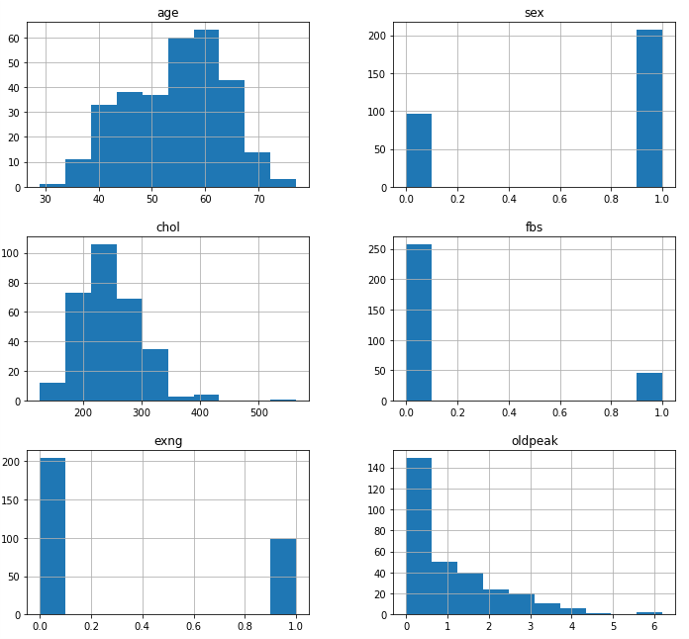
\includegraphics[width=13cm]{Data1.png}
    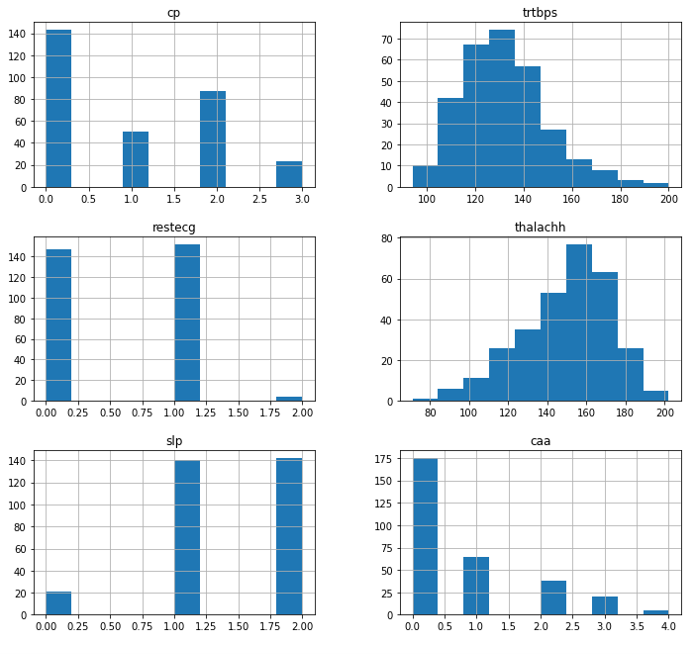
\includegraphics[width=13cm]{Data2.png}
\end{figure}
\begin{figure}[H]
    \centering
    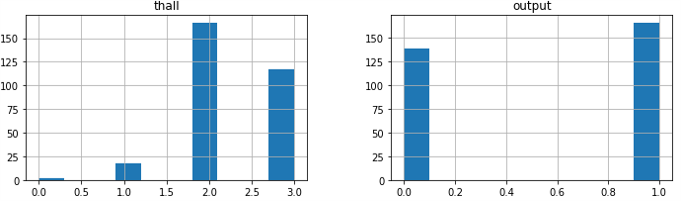
\includegraphics[width=13cm]{Data3.png}
\end{figure}
\noindent
Through the histograms, most of the features demonstrates a Gaussian distribution, only those that have binary values were unable to. We would like to see the correlations between each of the features and the output we are trying to predict. The following graphs shows the relations of the distributions in each feature between people that has less chance of heart attack and people that has more chance of heart attack.
\begin{figure}[H]
    \centering
    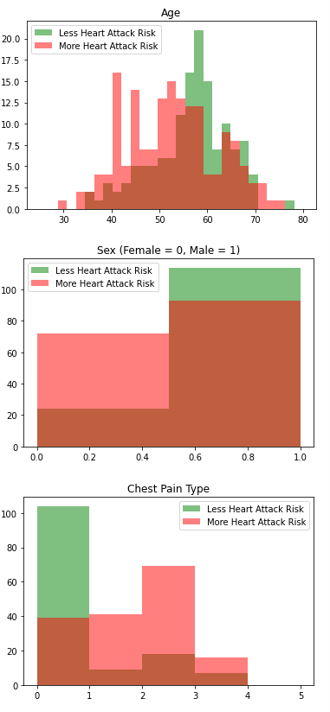
\includegraphics[width=7cm]{Corr1.png}
    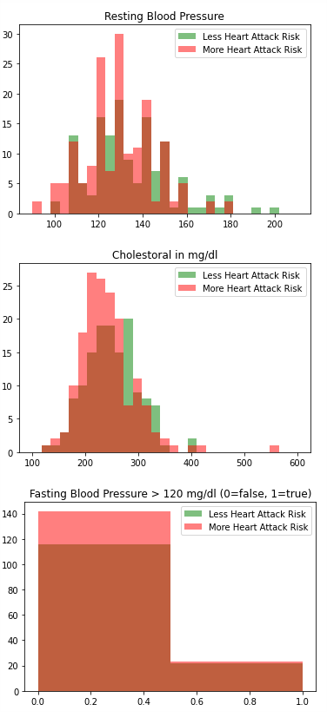
\includegraphics[width=7cm]{Corr2.png}
\end{figure}
\begin{figure}[H]
    \centering
    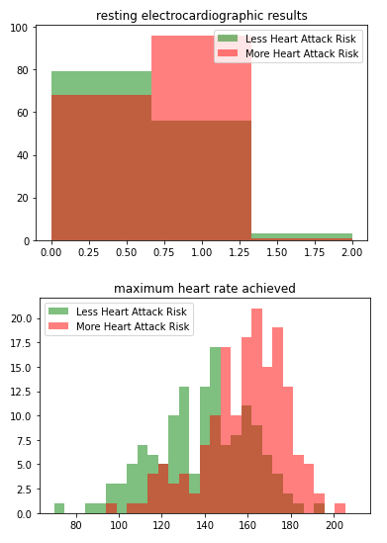
\includegraphics[width=7cm]{Corr3.png}
    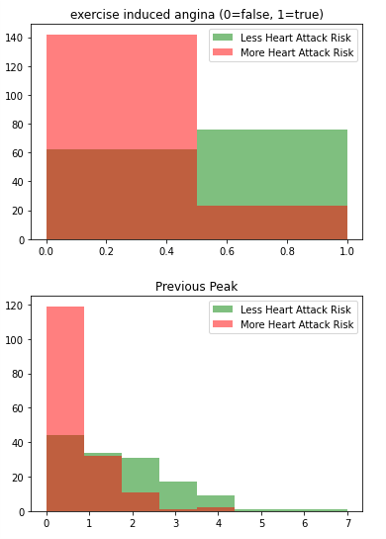
\includegraphics[width=7cm]{Corr4.png}
    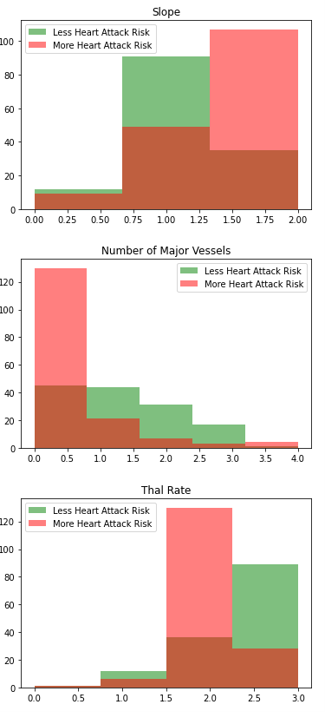
\includegraphics[width=7cm]{Corr5.png}
\end{figure}

In the graphs above, a green distribution shows the group that has less Heart Attack Rate, and a red distribution shows the group that has a more Heart Attack Rate. \\
Specifically, we see a very strong separation in the age category where people that are older shows a lesser chance of having an heart attack. This may seem unintuitive at first become we have been linking old age and heart attack all along. Perhaps it is because the specific group of younger people in the data set that has other features of showing heart attack.\\

In the case of resting blood pressure and fasting blood pressure, we see little difference between the two groups, which implies that they have little contribution in determining the output. \\

For data that shows a correlation, being female shows higher chance of heart attack; a higher Cholesterol shows a minor increased chance of having less Heart Attack Rate; having chest pain other than type 1 shows significant correlation for more Heart Attack Rate; resting electrocardiographic results of Value 1 shows more chance of Heart Attack Rate; not having exercise induced angina shows a correlation to having more Heart Attack Rate; higher maximum heart rate achieved shows significant correlation to higher Heart Attack Rate; having 0 previous peak shows strong correlation to more Heart Attack Rate; a slope value of 3 shows a correlation to higher Heart Attack rate; having less number of Vessels shows significant correlation to more Heart Attack Rate, and having less Thal Rate shows a strong correlation to more Heart Attack Rate.\\

Due to fact that resting/fasting blood pressure has little to do with the output, we could potentially eliminate them in the training of our models. And for other features that shows a strong or significant correlation, we could manually adjust them to have more initial weights and thus could significantly reduce the time to train. 
\section *{Regular Models}
Using the sklearn library, the code is run through the library provided functions for logistic regression, svms, and neural networks with essentially no regularization by giving it a high C value. The SVM is using a linear kernel, whereas for the neural network it has two hidden layers with 10 neurons each.\\\\The dataset is split into a training set and test set. The performance of the classifiers are given by the bar graph below, which depicts the accuracy when run against the training set and the test set. \\
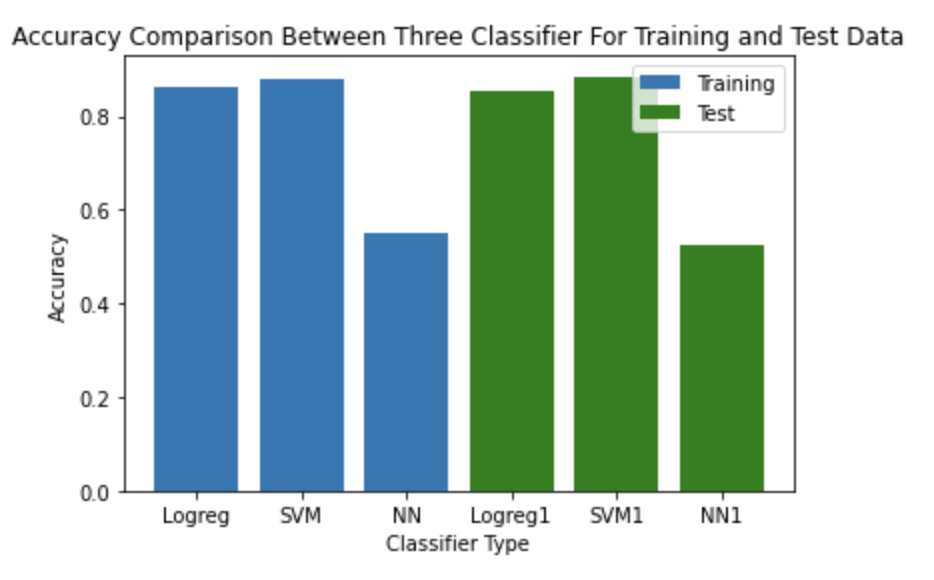
\includegraphics{1}\\
As shown by the graph, SVMs have the highest accuracy across both training and data sets. The similar accuracies between training data and test data maybe suggests that no overfitting has occurred, which is true across all three classifiers.\\
The logistic regression model follows closely behind, being only slightly outperformed whereas the neural network model seems to perform the worst, with barely 60\% accuracy even for the training set.

\section *{Modifications to Classifiers}
\subsection *{Modifications to Logistic Regression Model}
\subsubsection *{Adding L2 Regularization}
Adding L2 regularization to the logistic regression model seems to improve accuracy as c decreases. In our case when c=0.01 ($\lambda$ = 100), the test data accuracy is the highest, at almost 89\%. This may suggest that our unregularized model (arbitrarily high C) may be overfitting, and thus controlling the weights brings down the inaccuracy of the model.\\
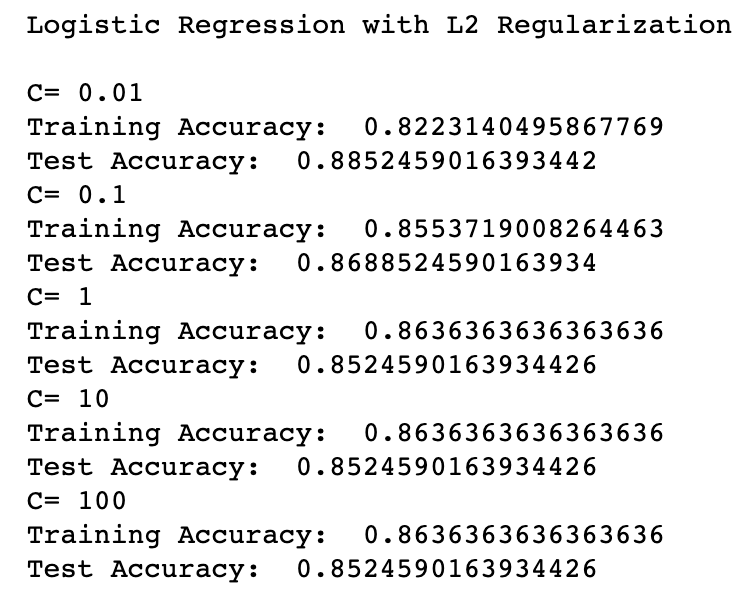
\includegraphics{2}\\\\
\subsubsection *{Polynomial Feature Transformation}
Performing polynomial feature transformations also yield improvements, but not as much as using L2 regularization. Polynomial transformation up to orders of 9 were tested, and is tested with logistic regression (without regularization). Test data accuracy fluctuates as $k$ increases, but peaks at $k$ = 6 when test accuracy equals ~86.9\%, which is an improvement over the untransformed features.\\
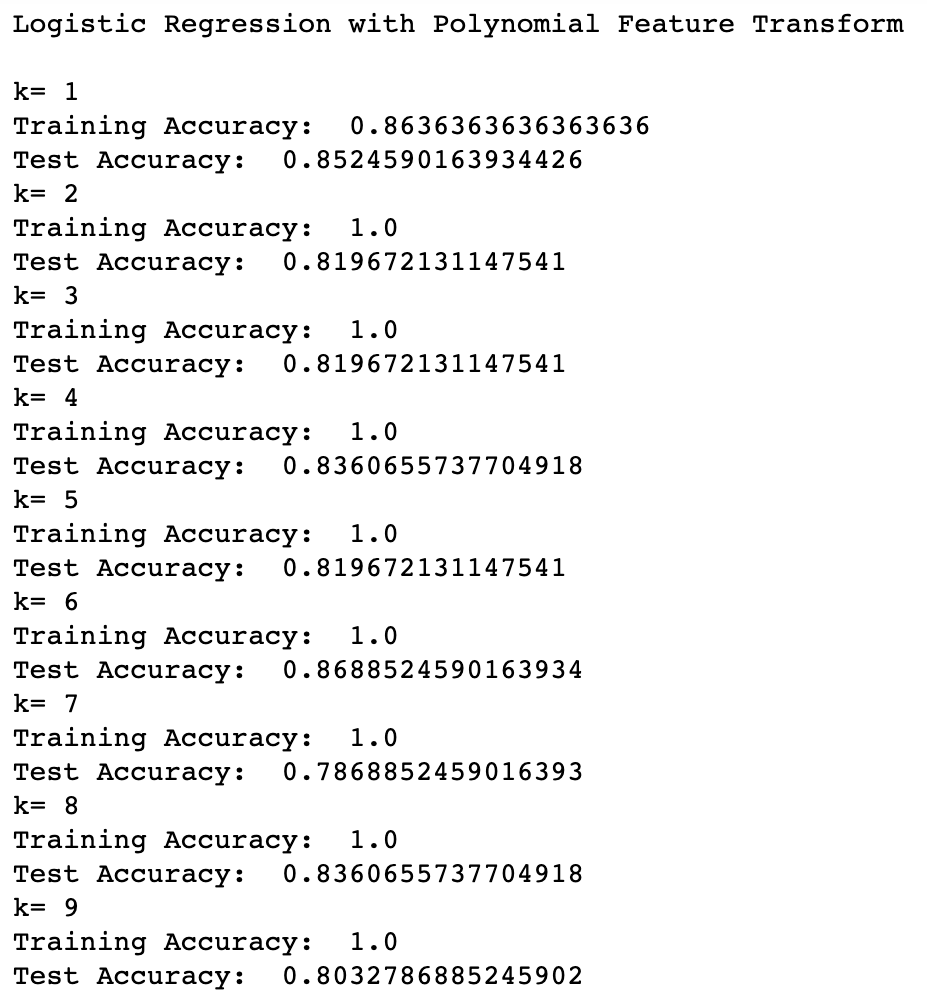
\includegraphics{3}\\\\
\subsection *{Modifications to SVM Model}
\subsubsection *{Adding L2 Regularization}
Adding L2 regularization to the Linear SVM model does not seem to change much. In fact, high regularization seems to make the model perform worse. This is expected, since having a very small margin essentially makes it a hard-margin SVM. This reveals something about the data set, in that it shows the dataset is not linearly separable. Thus, applying different kernels to the SVM may yield better results.\\
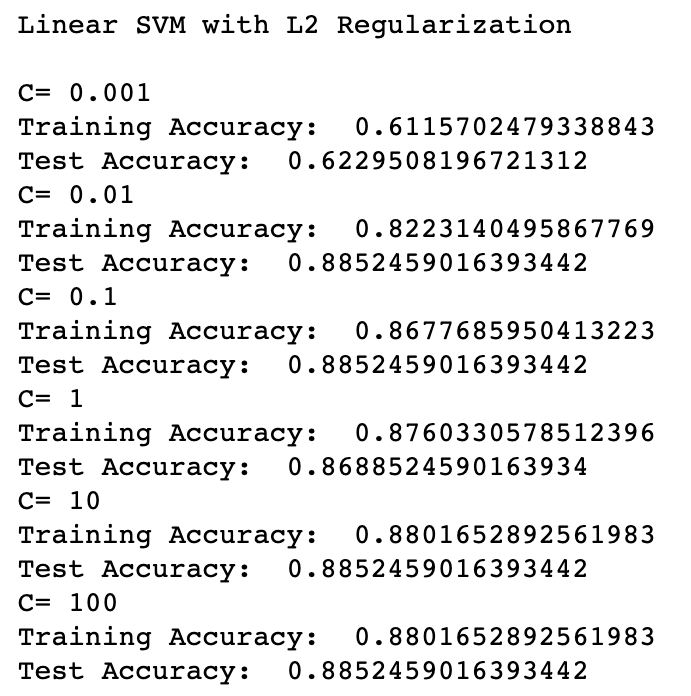
\includegraphics{4}\\
\subsubsection *{Radial Basis SVM}
RBF SVM does not seem to yield any improvements over linear SVM. However, something of note is that RBF SVM does have very high training accuracy, whereas test accuracy is more lackluster. This may suggest that RBF SVM may actually be overfitting.
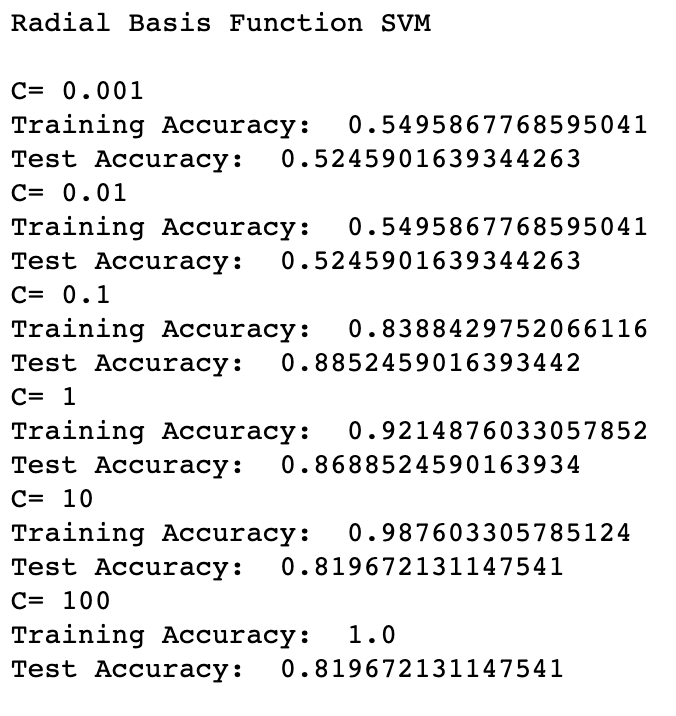
\includegraphics{5}\\
\subsubsection *{Polynomial SVM}
The polynomial yields the best test accuracy result (\~90\%) out of all the models tested. This may suggest that the polynomial kernel SVM may be the best fit model out of the three tested. However, note that when regularization is high (low C values) both training and test accuracy were low. This may suggest that the data is not linearly separable, and that a hard-margin SVM solution will not likely be possible.\\
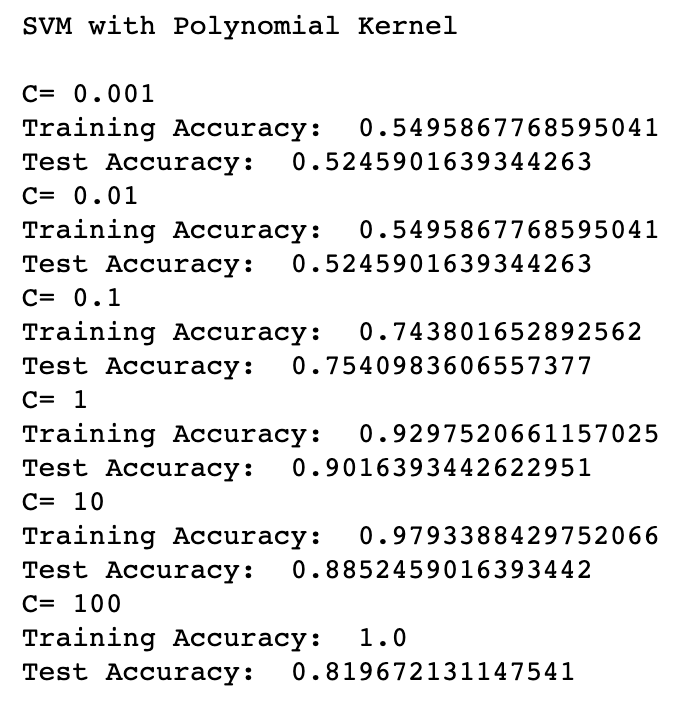
\includegraphics{6}
\subsection *{Modifications to Neural Network Model}
\subsubsection *{Adding L2 Regularization and Modifying Number of Layers}
Recall that the original setting is two layers with ten neurons each (10, 10). Adding regularization seems to have had a big impact, which suggests that without regularization, the data set may have been overfitting. \\
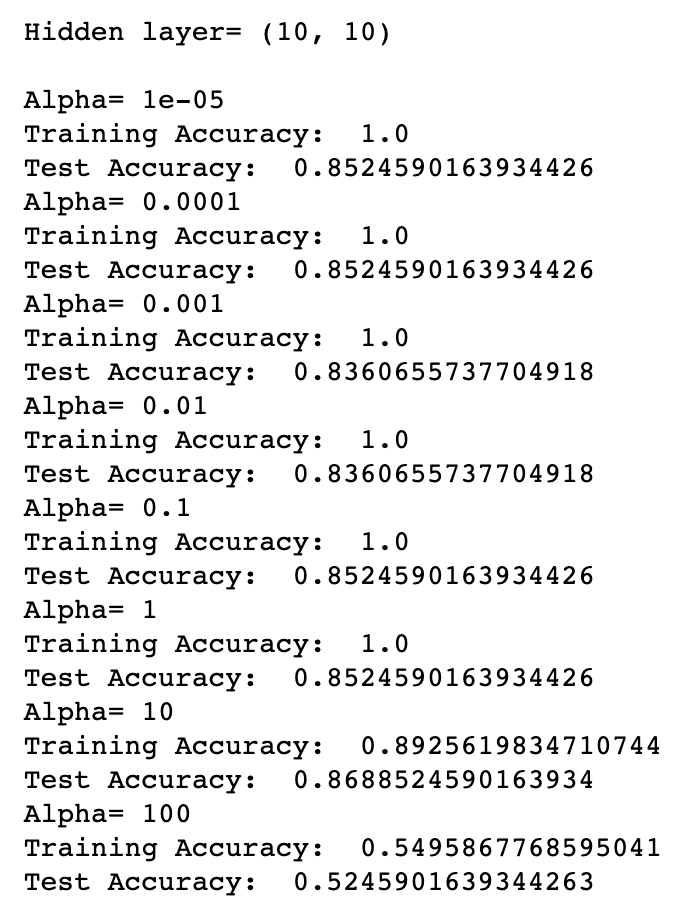
\includegraphics{7}\\
That said, adding/reducing layers does not seem to have much effect on the performance of the neural network. However, something of note is that when the neural network has only one hidden layer, the test accuracy for low regularization is significantly better when compared to neural networks with two and three layers, which may suggest that having more than one-layer may make regularization more important.\\
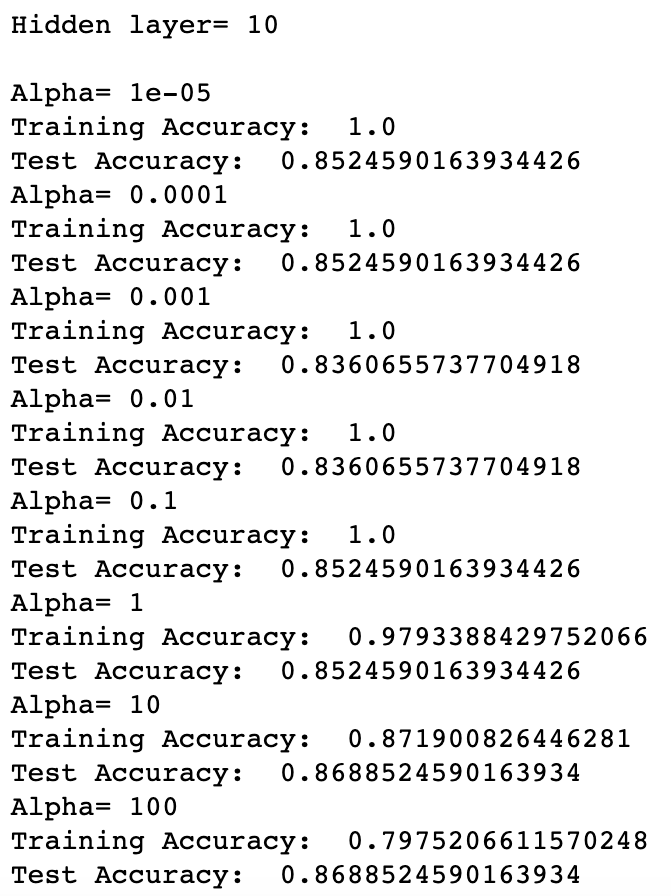
\includegraphics{8}\\
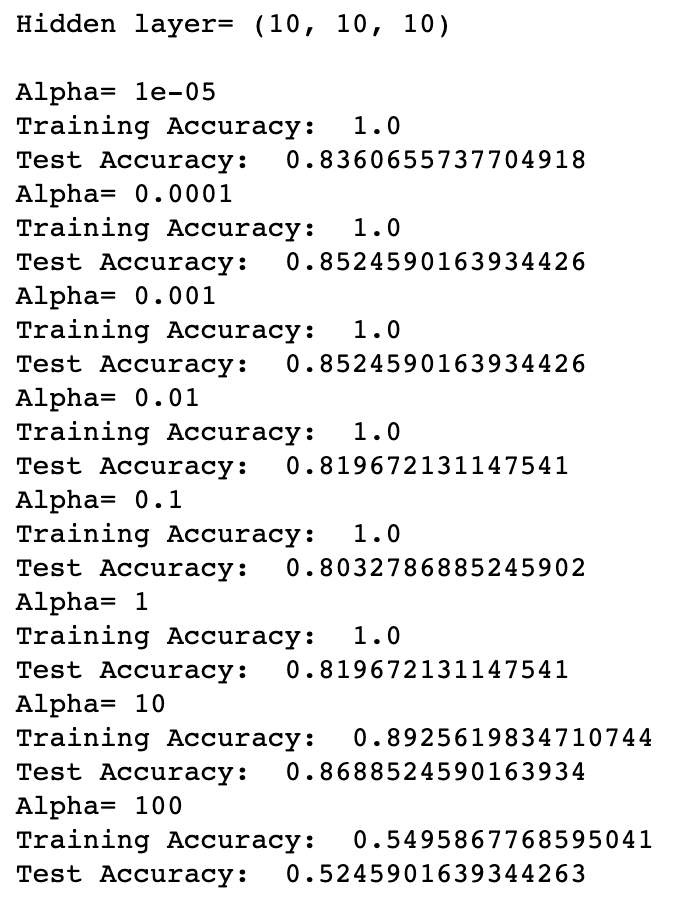
\includegraphics{9}\\

\section *{Conclusion}
Polynomial Kernel SVMs have the best performance overall, with moderate Regularization ($\lambda$=1). In fact, even with Linear SVMs and no other special modifications to the other classifiers, SVMs still perform better overall, with Logistic Regression models following closely behind. Therefore this result may suggest that the dataset may in fact be separable. However, decreasing c (increasing $\lambda$) in SVMs yielded worse performing models, thus we conclude that although results seem to suggest that the data is separable, it is not perfectly so, and thus cannot be solved by a hard-margin SVM. Therefore some leeway should be given to through less regularization to make it into a soft-margin SVM problem.\\\\
The mediocre performance of Neural Networks when regularization is low may suggest that having two-hidden layers already overfits the model, and thus regularization may be needed to penalize high weights. Apart from that, it may seem to suggest that having only one hidden layer would be sufficient for the neural network to perform similarly well to its counterparts with more layers, further bolstering the argument that neural networks have overfitted the model. 
\section *{Table of Results}
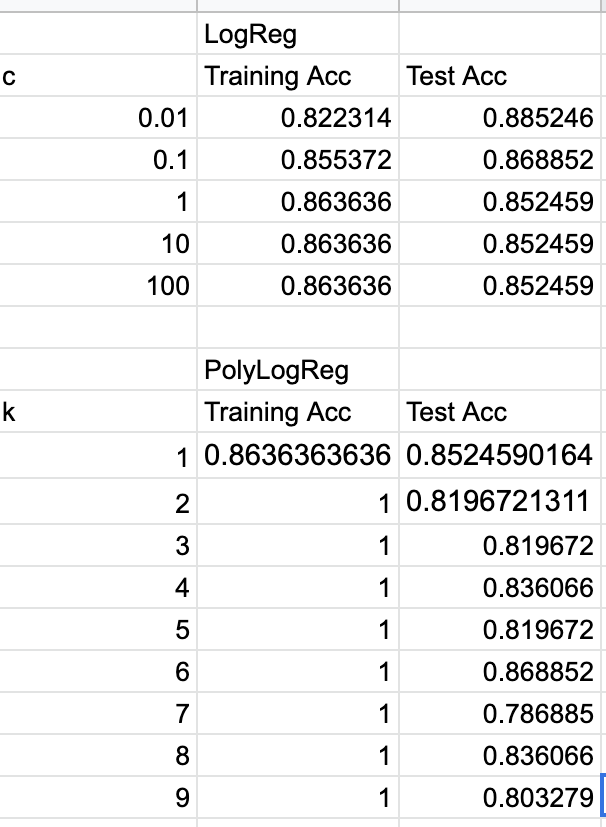
\includegraphics{10}\\\\
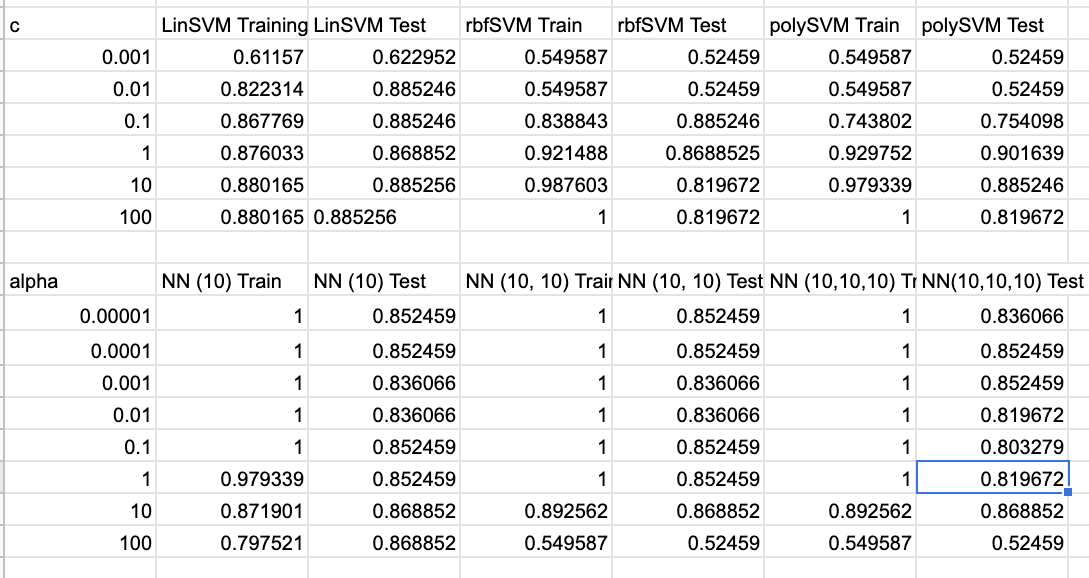
\includegraphics{11}[left]
\end{document}  